\documentclass[10pt]{scrartcl}
% \documentclass[10pt]{article}
\usepackage[T1]{fontenc}
\usepackage{amsmath,amsfonts,amssymb}
\usepackage{mathtools}
\usepackage{color,soul}
\usepackage{fullpage}
\usepackage{enumerate}
\usepackage{graphicx}
\usepackage[colorlinks=true,urlcolor=blue]{hyperref}
\usepackage{caption}
\usepackage{subcaption}
\usepackage{deluxetable}

\definecolor{Light}{gray}{.90}
\sethlcolor{Light}

\title{I Don't Care How Many Suns There Are}
\author{Jeren Suzuki}
\date{Last Edited \today}

\begin{document}

\maketitle
\pagenumbering{Roman}
\tableofcontents
\clearpage
\pagenumbering{arabic}

\section{Introdution} % (fold)
\label{sec:introdution}
    Now that we've got the \emph{basic} framework of finding the centers of 3 suns, let's make the code flexible enough to handle each scenario:\\
\begin{center}
    $\begin{matrix} 
    1 & 2 & 3 \\ 
    1 &   & 3 \\
    1 & 2 &   \\
      & 2 & 3 \\
    1 &   &   \\
      & 2 &   \\
      &   & 3
    \end{matrix}$
\end{center}

Where each row corresponds to a possibility of which regions will be in the image. this table already accounts for partial suns which we do not find centers of. 
% section introdution (end)

\section{Flexibilizing Our Code} % (fold)
\label{sec:flexibilizing_our_code}

As of now, the code only works with an image with regions 1, 2, and 3 as whole. The first step to make the code work under any condition is to create a workflow that efficiently makes decisions based on how many regions/what those regions are. The first step is to check if there are any partial suns, and if so, which. Once we have isolated which regions are center-friendly, we pass the region id(s) into the program. For example, for our current setup, we'd pass reg1, reg2, and reg3 as parameters in our program. There is a small problem however where in the current setup, the auxiliary regions depend on the position of the primary region. If for some reason the primary region is cut off, we're going to have some problems here.
% section flexibilizing_our_code (end)

\section{Dealing with < 3 suns} % (fold)
\label{sec:dealing_with_3_suns}
How do you tell the difference between 2 suns where one is $\approx 50$\% lower in intensity than the other? It is either a pair of region 1 and 2 suns or a pair of region 2 and 3 suns. Furthermore, how does one tell the difference from a region 1 and 2 sun that is somehow obscured to 50\% brightness and a region 2 and 3 sun at normal brightness? Unless there is a way to know whether or not something is artificially making the suns dimmer, it's hard. However, if we know that and we know the approximate thresholding, we can make guesses on which region is which.

For example, if we have 2 regions, 1 is 25\% the brightness of the other, we know that they are regions 1 and 3. If we only see 1 sun however, we must guess what the maximum should be and see at what percentage the max of the sun is (is it 25\%? 50\%?). This seems inefficient and should be improved. \\

Nicole suggests instead of using a foreknown number of suns we find the maxima of the 2nd deriv of the sorted array until we find no well-defined peaks. The problem with this approach is that we must define a ``well defined peak''. Figure \ref{reg12peaks} features the peaks of an image with the 100\% and 50\% sun which we try to take maximum of. Figure \ref{scaled12peaks} show that if we set some arbitrary thresholds, we can get the results we want. Now, how will those threshold hold up in different scenarios?


\begin{figure}[!h]
    \begin{center}
    \begin{subfigure}[b]{.49\textwidth}
        \centering
        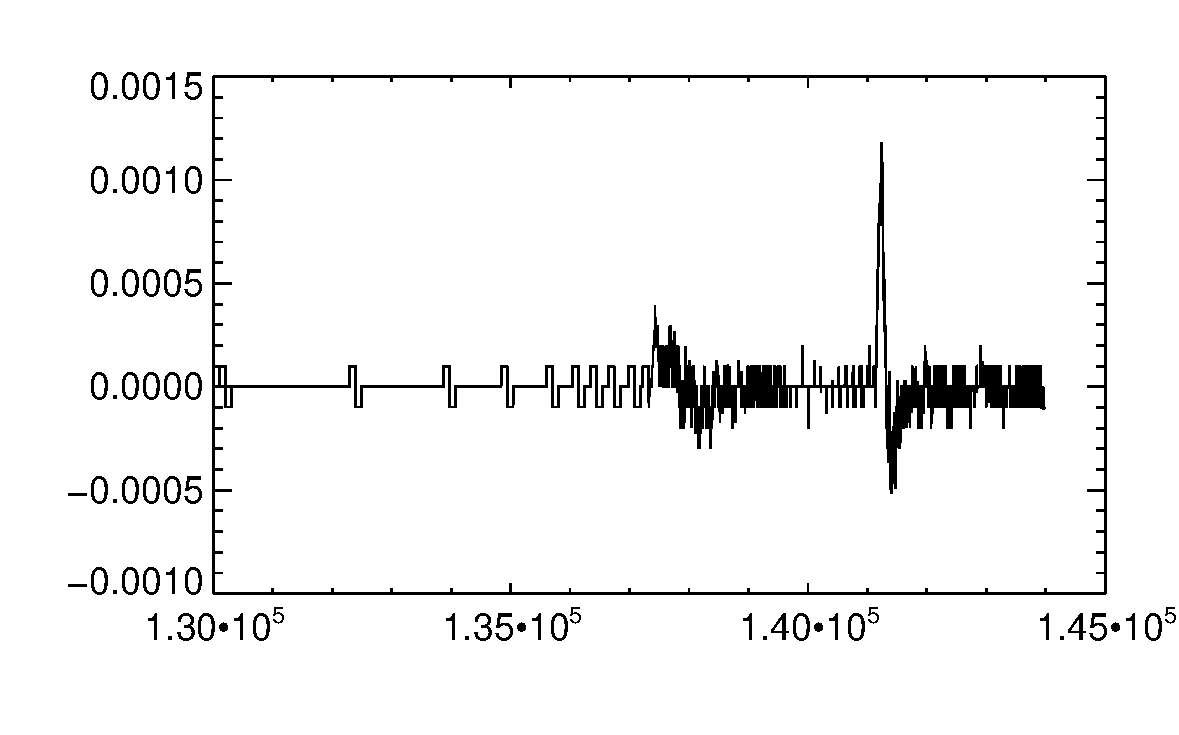
\includegraphics[width=1.\textwidth]{../plots_tables_images/reg12.eps}
        \caption{2nd deriv of sorred array}
        \label{reg12peaks}
    \end{subfigure}
    \begin{subfigure}[b]{.49\textwidth}
        \centering
        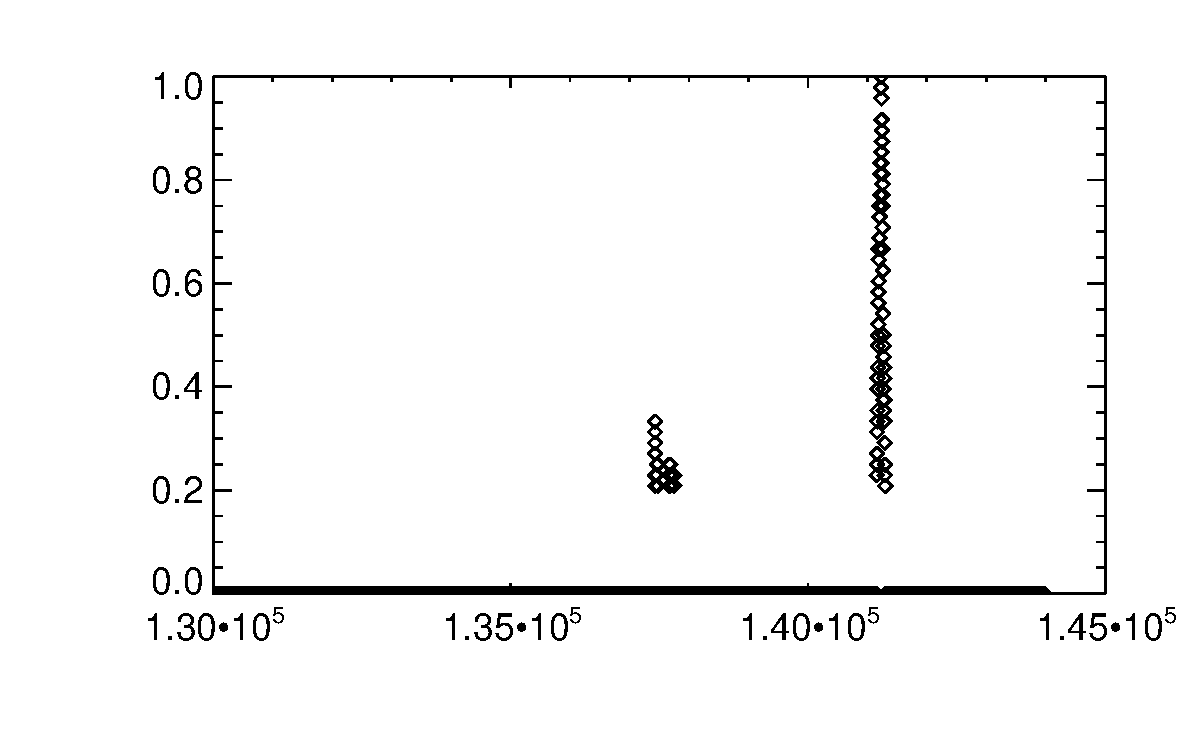
\includegraphics[width=1.\textwidth]{../plots_tables_images/scaledreg12.eps}
        \caption{Scaled positive values of 2nd deriv from 0 to 1, then thresholded to above .2}
        \label{scaled12peaks}
    \end{subfigure}

   \begin{subfigure}[b]{.49\textwidth}
        \centering
        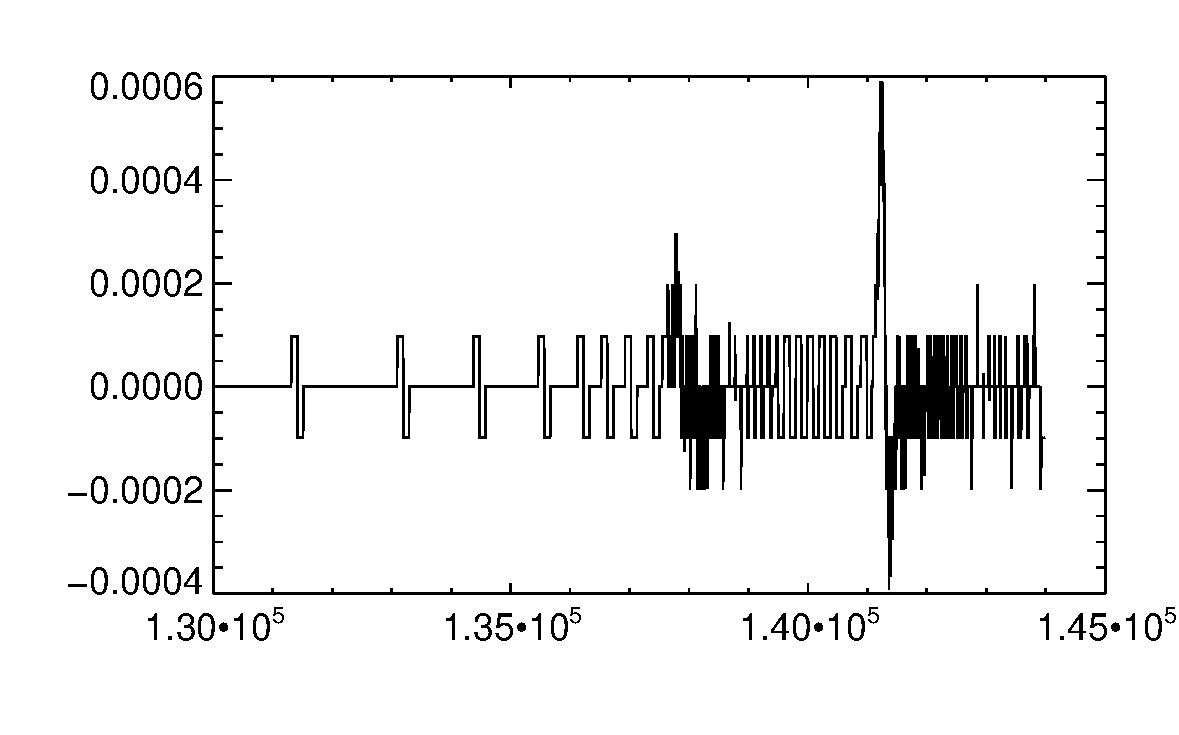
\includegraphics[width=1.\textwidth]{../plots_tables_images/reg23.eps}
        \caption{Now looking at the 50\% and 25\% sun}
        \label{reg23peaks}
    \end{subfigure}
    \begin{subfigure}[b]{.49\textwidth}
        \centering
        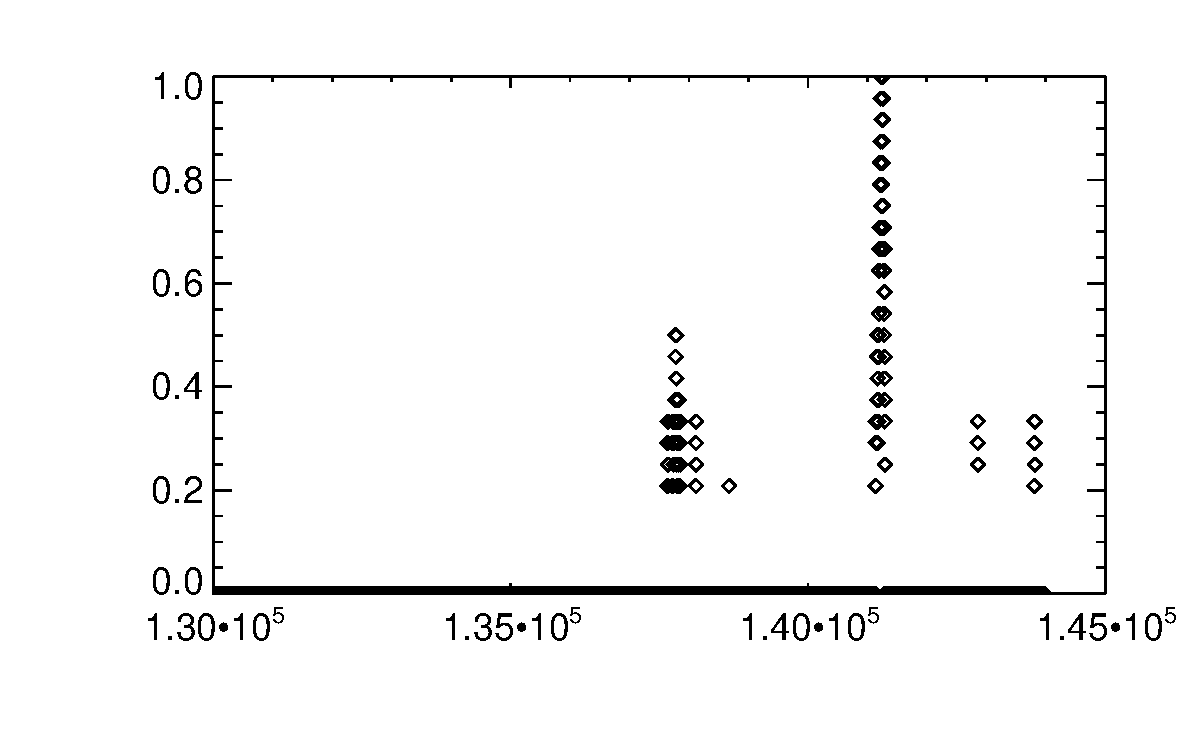
\includegraphics[width=1.\textwidth]{../plots_tables_images/scaledreg23.eps}
        \caption{}
        \label{scaled23peaks}
    \end{subfigure}
    \caption{}
    \end{center}
\end{figure}


If we look at the 50\% and 25\% brightness sun, we see in Figure \ref{scaled23peaks} that the same threshold which worked quite well in the first set of plots doesn't quite work well for others. The main problem is that we can find the maxima over and over, but we need to know when to stop. We can use \hl{\texttt{countsuns()}} to return the number of suns we have. Now the problem is that we don't know which peaks are for which suns. We cannot assume the highest peak is always the 100\% sun because there may be a case where only the 50\% and 25\% suns are available for centering. \\

Still working on this part. 


% section dealing_with_3_suns (end)

\section{Partial Suns} % (fold)
\label{sec:partial_suns}
Another big problem with identifying suns is how to deal with partial suns. We want to be able to take an image with 2 whole suns and 1 partial sun, eliminate the partial sun, and take the centers of the remaining regions. We accomplish this by:

\begin{enumerate}
    \item Reading in our image
    \item Scanning the border a certain length in to check for suns
    \item If any pixels are found, identify the partial sun as a mask and find the center of it
    \item Using the center position, zero-out a box of a certain length
    \item Return the fixed image with the partial sun removed
\end{enumerate}

Figure \ref{fixtheregion} shows the starting and ending product of the peocess to fix an image. The benefit of this approach (zero out) is the simplicity and speed. The other options were to operate on the starting image but ignore the partial area or to recrop the rest of the image.

\begin{figure}[!ht]
    \centering
   \begin{subfigure}[b]{.49\textwidth}
        \centering
        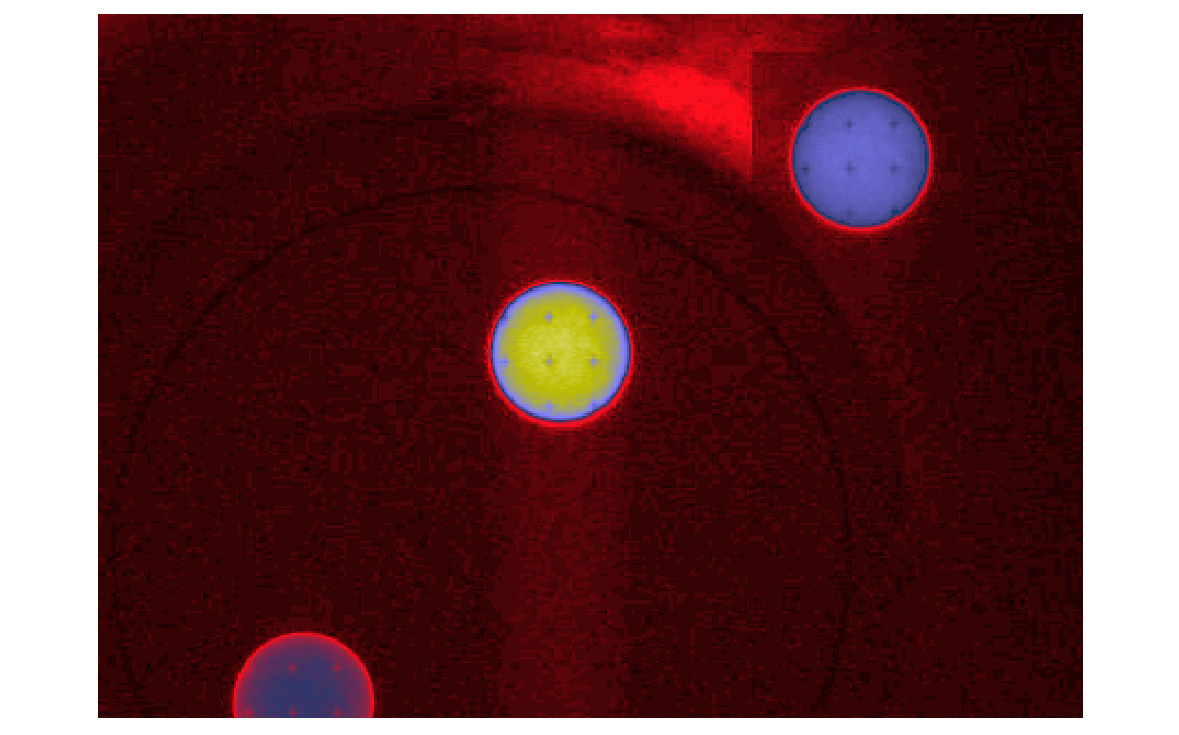
\includegraphics[width=1.\textwidth]{../plots_tables_images/inputimage.eps}
        \caption{Original image}
        \label{og_image}
    \end{subfigure}
    \begin{subfigure}[b]{.49\textwidth}
        \centering
        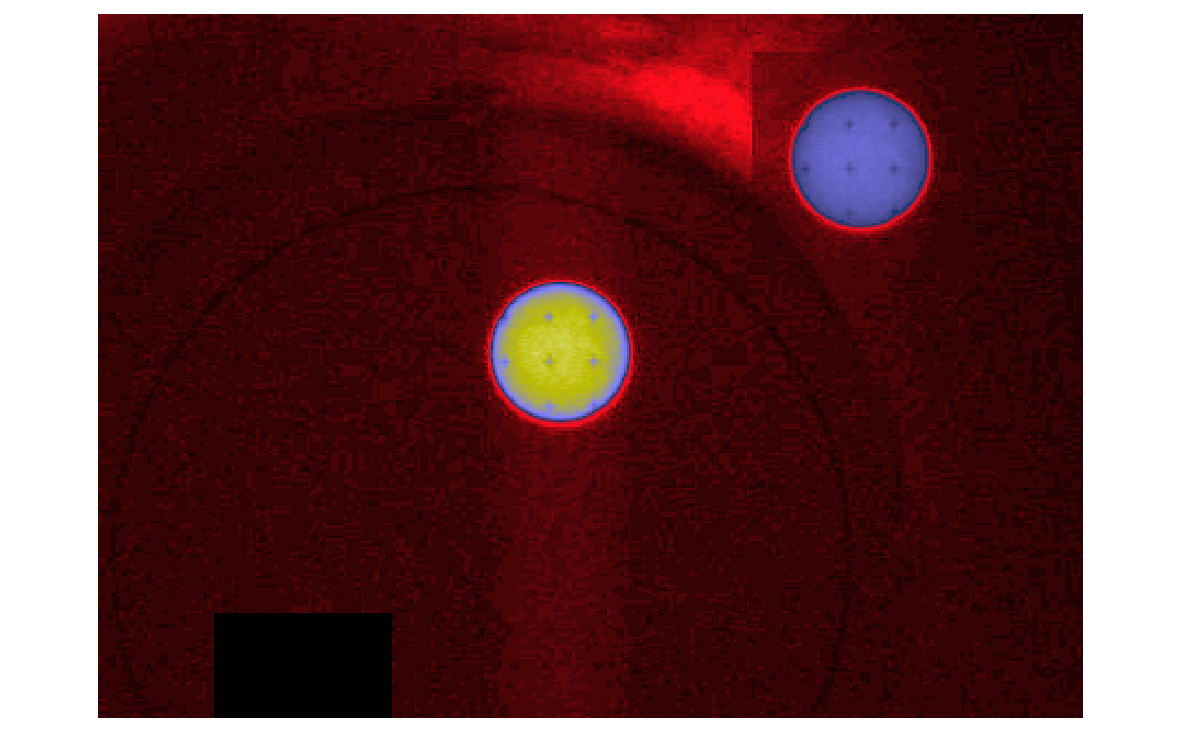
\includegraphics[width=1.\textwidth]{../plots_tables_images/fixedimage.eps}
        \caption{Image with the partial sun cropped out}
        \label{fixed_image}
    \end{subfigure}
    \caption{}
    \label{fixtheregion}
\end{figure}

The problem with this method is where it find the center of mass of the partial. If there are two partial suns, the center will not be on either of the suns and will possibly end up cropping a totally usable sun.
% section partial_suns (end)

\end{document}










